%%%%%%%%%%%%%%%%%%%%%%%%%%%%%%%%%%%%%%%%%%%%%%%%%%%%%%%%%%%%%%%%
%                                                              %
%                                                              %
% Macallyster S. Edmondson                                     %
%                                                              %
% ECE351-53                                                    %
%                                                              %
% Lab #3                                                       %
%                                                              %
% 02/01/2022                                                   %
%                                                              %
% Straigtforward layout, broken into sections, uses many       %
% common libraries. Note, Hyperlinks are not highlighted.      %
%                                                              %
%%%%%%%%%%%%%%%%%%%%%%%%%%%%%%%%%%%%%%%%%%%%%%%%%%%%%%%%%%%%%%%%

%%%%%%%%%%%%%%%%%%%%%%%%%%%%%%%%%%%%%%%%%%%
%%% DOCUMENT PREAMBLE %%%
\documentclass[12pt]{report}
\usepackage[english]{babel}
%\usepackage{natbib}
\usepackage{url}
\usepackage[utf8x]{inputenc}
\usepackage{amsmath}
\usepackage{graphicx}
\graphicspath{{./images/}}
\usepackage{parskip}
\usepackage{fancyhdr}
\usepackage{vmargin}
\usepackage{listings}
\usepackage[hidelinks]{hyperref}
\usepackage{xcolor}
\usepackage{datetime}
\usepackage[section]{placeins}
\definecolor{codegreen}{rgb}{0,0.6,0}
\definecolor{codegray}{rgb}{0.5,0.5,0.5}
\definecolor{codeblue}{rgb}{0,0,0.95}
\definecolor{backcolour}{rgb}{0.95,0.95,0.92}
\lstdefinestyle{mystyle}{
backgroundcolor=\color{backcolour},
commentstyle=\color{codegreen},
keywordstyle=\color{codeblue},
numberstyle=\tiny\color{codegray},
stringstyle=\color{codegreen},
basicstyle=\ttfamily\footnotesize,
breakatwhitespace=false,
breaklines=true,
captionpos=b,
keepspaces=true,
numbers=left,
numbersep=5pt,
showspaces=false,
showstringspaces=false,
showtabs=false,
tabsize=2
}
\lstset{style=mystyle}
\setmarginsrb{3 cm}{2.5 cm}{3 cm}{2.5 cm}{1 cm}{1 cm}{1 cm}{1.5 cm}
\title{Lab \#3 Report}
% Title
\author{Macallyster S. Edmondson}
% Author
\date{\today}
% Date
\makeatletter
\let\thetitle\@title
\let\theauthor\@author
\let\thedate\@date
\makeatother
\pagestyle{fancy}
\fancyhf{}
\rhead{\theauthor}
\lhead{\thetitle}
\lfoot{Page: \thepage}
\rfoot{\thedate}
\fancypagestyle{customplain}{ %Used for default pages with plain style to keep overall document consistency
  \fancyhf{}
  \renewcommand{\headrulewidth}{0pt} %Remove bar from top of page
  \lfoot{Page: \thepage}
}
\fancypagestyle{titlepage}{ %Used for default pages with plain style to keep overall document consistency
  \fancyhf{}
  \renewcommand{\headrulewidth}{0pt} %Remove bar from top of page
  \cfoot{\thedate}
}
%%%%%%%%%%%%%%%%%%%%%%%%%%%%%%%%%%%%%%%%%%%%
\begin{document}
%%%%%%%%%%%%%%%%%%%%%%%%%%%%%%%%%%%%%%%%%%%%%%%%%%%%%%%%%%%%%%%%%%%%%%%%%%
%%%%%%%%%%%%%%%
\begin{titlepage}\thispagestyle{titlepage}
\centering
%\vspace*{0.5 cm}

\includegraphics[scale = 0.12]{univ-logo.png}\\[1.0 cm]
%University of Idaho
\begin{center}    \textsc{\Large   ECE 351 - Section \#53 }\\[2.0 cm]
\end{center}% University Name

%Lab Report
\rule{\linewidth}{0.2 mm} \\[0.4 cm]
{ \huge \bfseries \thetitle}\\
\rule{\linewidth}{0.2 mm} \\[0.5 cm]
\textsc{\Large Discrete Convolution }\\[1.5 cm] % Course 
\begin{minipage}{0.4\textwidth}
\begin{flushleft} \large
\emph{Submitted To:}\\
Kate Antonov\\ \small
University of Idaho\\
kantonov@uidaho.edu\\
\hfill
\end{flushleft}
\end{minipage}~
\begin{minipage}{0.4\textwidth}
\begin{flushright} \large
\emph{Submitted By :} \\
\theauthor \\ \small
University of Idaho\\
edmo7033@vandals.uidaho.edu\\
\href{http://github.com/mac-edmondson}{github.com/mac-edmondson}\\
\end{flushright}
\end{minipage}\\[2 cm]
\vfill
\end{titlepage}
%%%%%%%%%%%%%%%%%%%%%%%%%%%%%%%%%%%%%%%%%%%%%%%%%%%%%%%%%%%%%%%%%%%%%%%%%%
%%%%%%%%%%%%%%%
\tableofcontents\thispagestyle{customplain}
\pagebreak
%%%%%%%%%%%%%%%%%%%%%%%%%%%%%%%%%%%%%%%%%%%%%%%%%%%%%%%%%%%%%%%%%%%%%%%%%%
%%%%%%%%%%%%%%%
\renewcommand{\thesection}{\arabic{section}}
\section{Introduction}
The goal of this lab was to become familiar with discrete convolutions using Python. This was a great lab for finding a deeper understanding of the summation definition
of a convolution. In order to complete this lab, the Python programming language was used with the \textit{Spyder-IDE} downloaded using \textit{Python Anaconda3}. The packages used in the 
completion of this lab were \texttt{numpy} for definitions of mathematical functions, \texttt{matplotlib.pyplot} to plot outputs of functions, and \texttt{scipy.signal} to verify the 
operation of the convolution function I implemented. 

All code for this lab, including this report, can be found on \href{http://github.com/mac-edmondson}{my Github}.
\section{Equations}
The equations used within this lab are shown in this section. The equations will be referenced by number throughout the rest of the report.
\begin{equation}\label{eq: 1}
  \begin{aligned}[c]
    f_1(t) = u(t-2) - u(t-9)\\
  \end{aligned}
\end{equation}
\begin{equation}\label{eq: 2}
  \begin{aligned}[c]
    f_2(t) = e^{-t} u(t)
  \end{aligned}
\end{equation}
\begin{equation}\label{eq: 3}
  \begin{aligned}
    f_3(t) = r(t-2) [u(t-2)-u(t-3)] + r(4-t) [u(t-3) - u(t-4)]
  \end{aligned}
\end{equation}

\section{Methodology}
\subsection{Lab: Part 1}
In Part 1 of this lab, the goal was to implement Equations \eqref{eq: 1}, \eqref{eq: 2}, \eqref{eq: 3} and plot the output. This was just like code seen from 
previous labs for function implementations. The code for this part of the lab can be seen below and the graph can be seen in Figure \ref{fig: p1t2}. Code for 
plot generation is not shown. 
\begin{lstlisting}[language=Python, basicstyle=\footnotesize]
    #PART 1
    #1
    def f1(t) :
        y = ss.u(t - 2) - ss.u(t-9);
        return y;
    
    def f2(t) :
        y = np.exp(-t) * ss.u(t)
        return y
    
    def f3(t) :
        y = (ss.r(t-2) * (ss.u(t-2) - ss.u(t-3))) + (ss.r(4-t) * (ss.u(t-3) - ss.u(t-4)))
        return y

    #Plot...
\end{lstlisting}
\subsection{Lab: Part 2}
In Part 2 of this lab, the goal was to implement a discrete convolution function to take and graph the convolution of a combination of the functions from Part 1. 
As discussed later in this report, implementing this function was very challenging and without the help of my peers and the Lab TA, it would have taken me much longer
to complete this part of the lab. The function defined is based on the summation definition of a convolution of two functions. Seen below is the code implemented for
Part 2 of this lab, excluding the code for graph output. 
\begin{lstlisting}[language=Python, basicstyle=\footnotesize]
  #PART 2

  #1
      
  def my_conv(f1, f2):
      Nf1 = len(f1)
      Nf2 = len(f2)
      f1Ex = np.append(f1, np.zeros((1, Nf2-1)))
      f2Ex = np.append(f2, np.zeros((1, Nf1-1)))
      result = np.zeros(f1Ex.shape)
      for i in range(Nf2 + Nf1 - 2) :
          result[i] = 0
          for j in range(Nf1):
              if(i-j+1 > 0):
                      try:
                          result[i] += f1Ex[j]*f2Ex[i-j+1]
                      except:
                          print(i, j)
      return result

  bound = 20
  t = np.arange(0, bound + step_size, step_size)
  f1 = f1(t)
  f2 = f2(t)
  f3 = f3(t)
  f1f2m = my_conv(f1, f2)
  f2f3m = my_conv(f2, f3)
  f1f3m = my_conv(f1, f3)
  t = np.arange(0, bound*2 + step_size, step_size)

  #Plot...
\end{lstlisting}

\section{Results}
The results of this lab are very straightforward. The implementation of all functions worked as expected and there is not much to discuss that wasn't covered in the Methodology 
Section of this report. 

The deliverables for Parts 1 \& 2 of this lab can be seen in Figures \ref{fig: p1t2} and \ref{fig: p2t2}, below.
\\
\begin{figure}[h!]
  \centering
  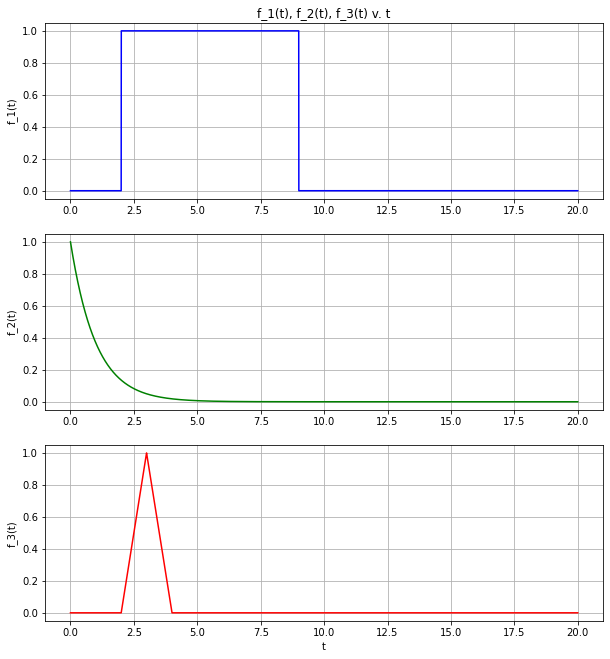
\includegraphics[scale=0.5]{p1t2.png}
  \caption{Part 1, Task 2 - Plots of Python Implementations of \eqref{eq: 1}, \eqref{eq: 2}, \eqref{eq: 3}}
  \label{fig: p1t2}
\end{figure}
\begin{figure}[h!]
  \centering
  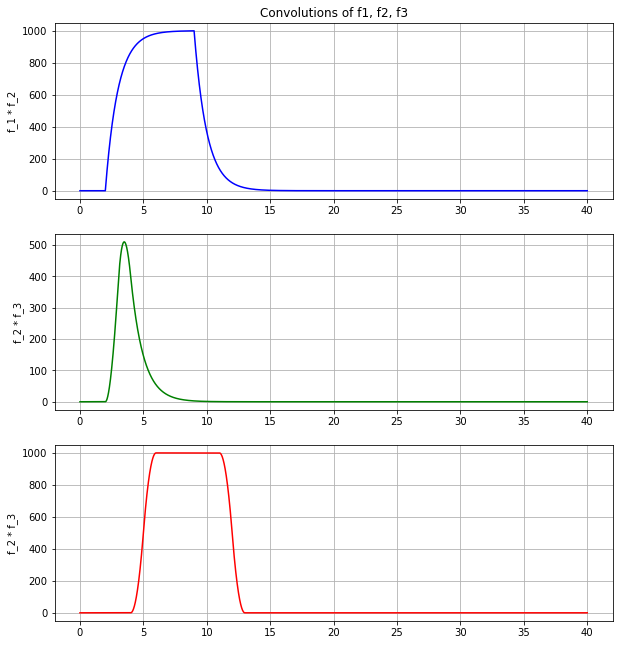
\includegraphics[scale=0.5]{p2t2.png}
  \caption{Part 2, Task 2 - Convolutions of Functions from Part 1, Task 2}
  \label{fig: p2t2}
\end{figure}
\section{Error Analysis}
The main problem faced during this lab was the implementation of the discrete convolution function itself. With many tried and failed attempts of the implementation
of this function, it is a wonder I got it working. I would not have got my function working without the lab discussion that took place to go in depth on the definition
of a convolution. Other than this, all of the basic implementation of functions and plotting with python were very straightforward.
\section{Questions}
\begin{itemize}
  \item I did not work alone during this lab. For majority of the lab session I attempted to collaborate with class mates to come up with a solution, though it wasn't
  until the class discussion that the solution came out.
  \item The most difficult part of this lab was implementing the discrete convolution function. Most of my useful problem solving came from putting ideas on a white board
  but even this did not push me to the solution until a class discussion.
  \item During my problem solving, I thought it was easiest to think about a graphical convolution but I did look at the analytical definition within the class textbook.
  The graphical approach was a lot simpler for my mind to grasp as compared to the analytical approach.
  \item This lab and its tasks were very concise in what is expected for deliverables.
\end{itemize}
\section{Conclusion}
In conclusion, I feel this lab was very successful. No doubt, this was a very difficult lab but I think my understanding of convolutions is better after studying the code
for some time. I am continuing to enjoy using Python to perform discrete calculus. For feedback, I would say it would be very helpful if the summation definition of a
convolution was given in the lab handout, even if it was a reference to a reading on the topic. Other than this, this was a great lab!
\newpage
% \begin{thebibliography}{111}
% \thispagestyle{customplain}

% \end{thebibliography}
\end{document}
%This template was created by Roza Aceska.